\begin{figure}[h!]
\centering
\begin{minipage}[b]{0.45\linewidth}
    \centering
    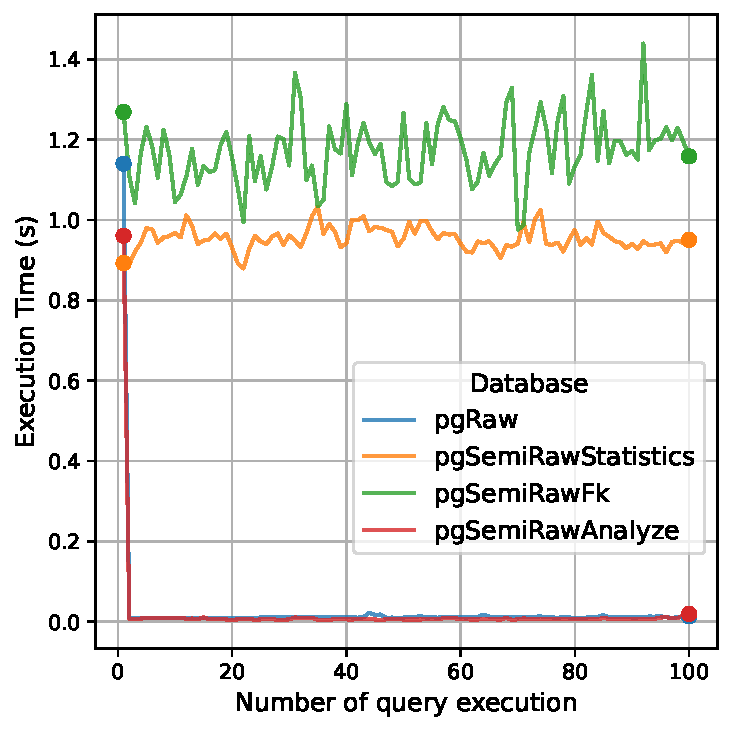
\includegraphics[width=1.0\linewidth]{charts-eval-exp-time-stat/execution_time_db_type_Q1.pdf}
    \caption*{Q1}
\end{minipage}
\hfill
\begin{minipage}[b]{0.45\linewidth}
    \centering
    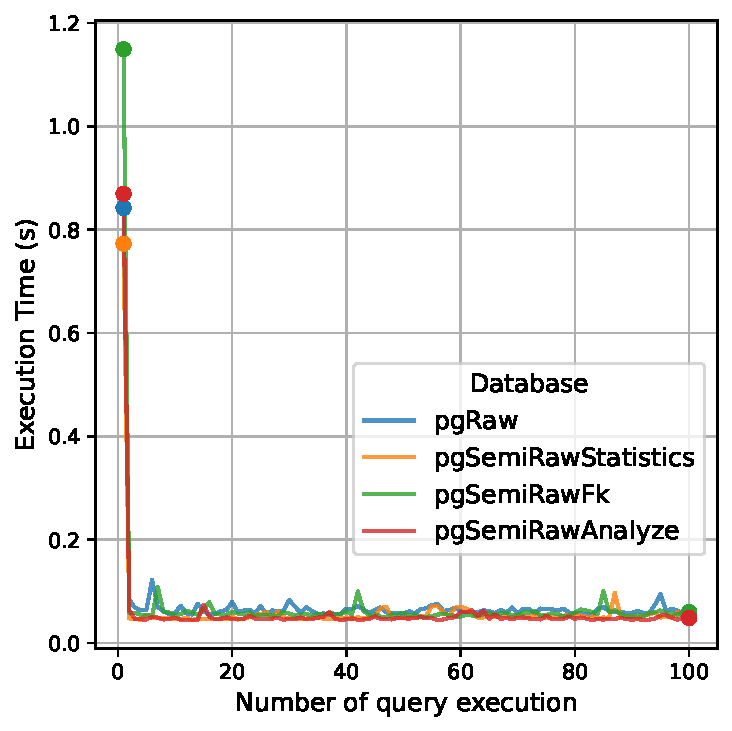
\includegraphics[width=1.0\linewidth]{charts-eval-exp-time-stat/execution_time_db_type_Q2.pdf}
    \caption*{Q2}
\end{minipage}
\vspace{0.5cm}
\begin{minipage}[b]{0.45\linewidth}
    \centering
    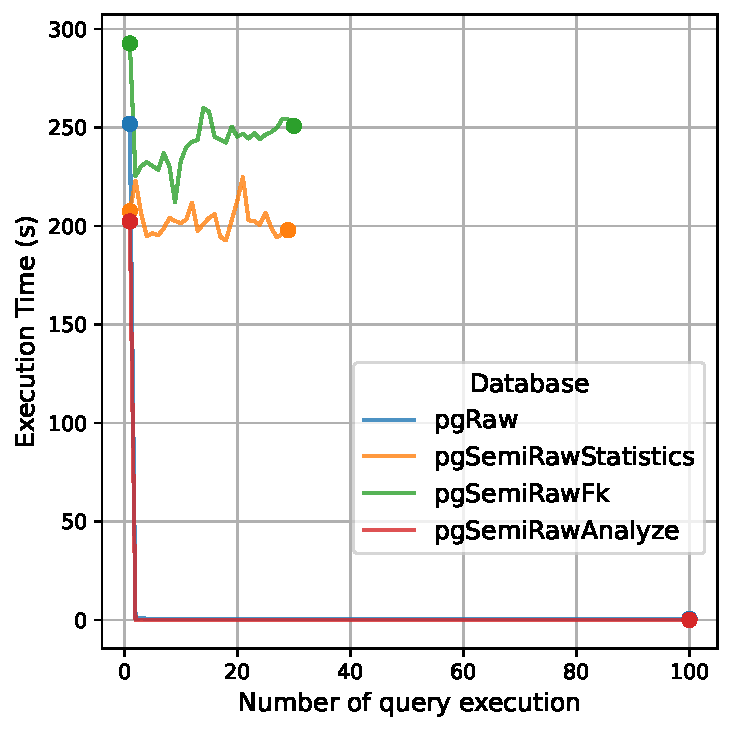
\includegraphics[width=1.0\linewidth]{charts-eval-exp-time-stat/execution_time_db_type_Q3.pdf}
    \caption*{Q3}
\end{minipage}
\hfill
\begin{minipage}[b]{0.45\linewidth}
    \centering
    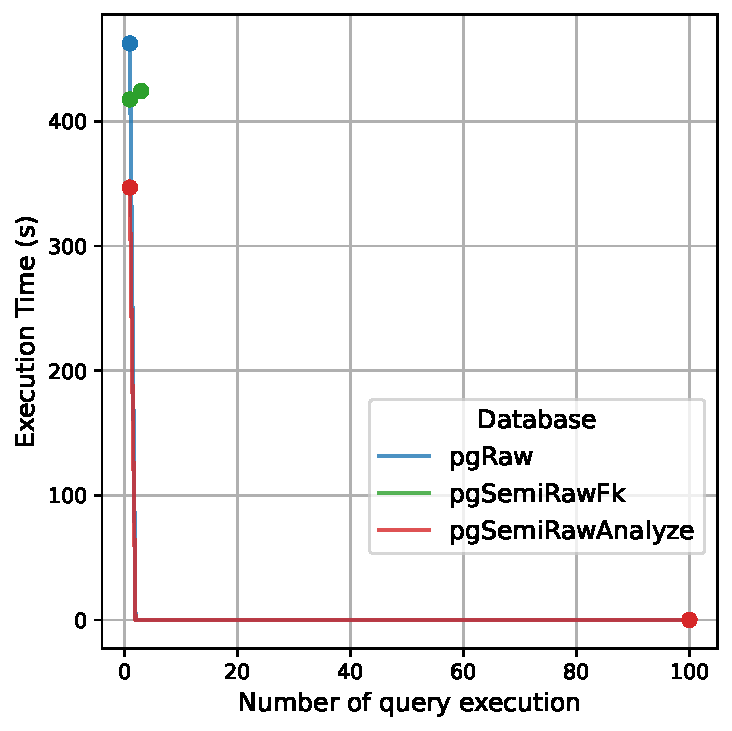
\includegraphics[width=1.0\linewidth]{charts-eval-exp-time-stat/execution_time_db_type_Q4.pdf}
    \caption*{Q4}
\end{minipage}
\caption[The execution times for queries Q1, Q2, Q3, and Q4 over 100 iterations]{The execution times for queries Q1, Q2, Q3, and Q4 over 100 iterations, utilising various types of PostgresSemiRaw, each with different levels of statistics metadata and PostgresRaw. These databases include TPC-H data with the \acrshort{sf} 0.1 alongside different levels of metadata.}
\label{fig:execution_time_stat_group1}
\end{figure}
